%%
%% This is file `sample-sigconf.tex',
%% generated with the docstrip utility.
%%
%% The original source files were:
%%
%% samples.dtx  (with options: `sigconf')
%% 
%% IMPORTANT NOTICE:
%% 
%% For the copyright see the source file.
%% 
%% Any modified versions of this file must be renamed
%% with new filenames distinct from sample-sigconf.tex.
%% 
%% For distribution of the original source see the terms
%% for copying and modification in the file samples.dtx.
%% 
%% This generated file may be distributed as long as the
%% original source files, as listed above, are part of the
%% same distribution. (The sources need not necessarily be
%% in the same archive or directory.)
%%
%% The first command in your LaTeX source must be the \documentclass command.
\documentclass[sigconf]{acmart}
\usepackage{algorithm}
\usepackage{algorithmicx}
\usepackage{algpseudocode}
\usepackage{graphicx}
\usepackage{caption}
\usepackage{subcaption}

%%
%% \BibTeX command to typeset BibTeX logo in the docs
\AtBeginDocument{%
  \providecommand\BibTeX{{%
    \normalfont B\kern-0.5em{\scshape i\kern-0.25em b}\kern-0.8em\TeX}}}

%% Rights management information.  This information is sent to you
%% when you complete the rights form.  These commands have SAMPLE
%% values in them; it is your responsibility as an author to replace
%% the commands and values with those provided to you when you
%% complete the rights form.
\setcopyright{acmcopyright}
\copyrightyear{2020}
\acmYear{2020}
\acmDOI{10.1145/3185768.3186313}

%% These commands are for a PROCEEDINGS abstract or paper.
\acmConference[ICPE `20]{ICPE `20: ACM/SPEC International Conference on Performance Engineering}{April 20--24, 2020}{Edmonton, Canada}
\acmBooktitle{ICPE `20: ACM/SPEC International Conference on Performance Engineering,
  April 20--24, 2020, Edmonton, Canada}
\acmPrice{15.00}
\acmISBN{978-1-4503-XXXX-X/18/06}


%%
%% Submission ID.
%% Use this when submitting an article to a sponsored event. You'll
%% receive a unique submission ID from the organizers
%% of the event, and this ID should be used as the parameter to this command.
%%\acmSubmissionID{123-A56-BU3}

%%
%% The majority of ACM publications use numbered citations and
%% references.  The command \citestyle{authoryear} switches to the
%% "author year" style.
%%
%% If you are preparing content for an event
%% sponsored by ACM SIGGRAPH, you must use the "author year" style of
%% citations and references.
%% Uncommenting
%% the next command will enable that style.
%%\citestyle{acmauthoryear}

%%
%% end of the preamble, start of the body of the document source.
\begin{document}
\emergencystretch 3em

%%
%% The "title" command has an optional parameter,
%% allowing the author to define a "short title" to be used in page headers.
\title{Optimizing carbon tax for decentralized electricity markets using an agent-based model}

%%
%% The "author" command and its associated commands are used to define
%% the authors and their affiliations.
%% Of note is the shared affiliation of the first two authors, and the
%% "authornote" and "authornotemark" commands
%% used to denote shared contribution to the research.
%\author{Alexander Kell}
%\affiliation{%
%  \department{School of Computing}
%  \institution{Newcastle University}
%  \city{Newcastle upon Tyne}
%  \country{UK}
%}
%\email{a.kell2@newcastle.ac.uk}
%
%\author{A. Stephen McGough}
%\affiliation{%
%  \department{School of Computing}
%  \institution{Newcastle University}
%  \city{Newcastle upon Tyne}
%  \country{UK}
%}
%\email{stephen.mcgough@newcastle.ac.uk}
%
%\author{Matthew Forshaw}
%\affiliation{%
%  \department{School of Computing}
%  \institution{Newcastle University}
%  \city{Newcastle upon Tyne}
%  \country{UK}
%}
%\email{matthew.forshaw@newcastle.ac.uk}
\author{Anonymized}
%%
%% By default, the full list of authors will be used in the page
%% headers. Often, this list is too long, and will overlap
%% other information printed in the page headers. This command allows
%% the author to define a more concise list
%% of authors' names for this purpose.
\renewcommand{\shortauthors}{Anonymized}
%\renewcommand{\shortauthors}{Kell et al.}

%%
%% The abstract is a short summary of the work to be presented in the
%% article.
\begin{abstract}
 
 Placeholder
 
\end{abstract}

%%
%% The code below is generated by the tool at http://dl.acm.org/ccs.cfm.
%% Please copy and paste the code instead of the example below.
%%


%%
%% Keywords. The author(s) should pick words that accurately describe
%% the work being presented. Separate the keywords with commas.
\keywords{Energy markets, policy, carbon tax, genetic algorithm, optimization, digital twin, agent-based models, electricity market model}

%% A "teaser" image appears between the author and affiliation
%% information and the body of the document, and typically spans the
%% page.


%%
%% This command processes the author and affiliation and title
%% information and builds the first part of the formatted document.
\maketitle

\section{Introduction}


% Computer simulation - why it is required

Computer simulation allows practitioners to model real-world systems using software. These simulations allow for `\textit{what-if}' analyses which can provide an indication as to how a system may behave under certain policies, environments and assumptions. These simulations become particularly important in systems which have high costs, impacts or risks associated with them.

% Electricity markets

Electricity markets are an example of such a system. Disruptions to electricity supply, a substantial increase in the cost of electricity or unrestrained carbon emissions have the potential to destabilise economies. It is for reasons such as these that electricity market models are used to test hypotheses, develop strategies and gain an understanding of underlying dynamics to prevent undesirable consequences \cite{Jebaraj2006}. 

In this paper we use the electricity market agent-based model ElecSim to find an optimum carbon tax strategy \cite{Kell}. Specifically, we use a genetic algorithm to find a carbon tax policy to reduce both average electricity price and the relative carbon density by 2035 for the UK electricity market. 

Carbon taxes have been shown to lower emissions quickly with lower costs to the public, with no upper bounds in terms of the reduction potential \cite{Wittneben2009}. Carbon taxes are able to send clear price signals, as opposed to a cap-and-trade scheme, such as the EU Emissions Trading System, which has shown to be unstable.

In this paper we use the reference scenario projected by the UK Government's Department for Business \& Industrial Strategy (BEIS) and used the model parameters calibrated by Kell \textit{et al.} \cite{DBEIS2019,Kell2020}. This reference scenario projects energy and emissions until 2035. We undertook various carbon tax policy interventions to see how we could reduce relative carbon density whilst at the same time reduce the average electricity price.


In contrast to grid or random search, genetic algorithms have the ability to converge on an optimal solution by trialling a fewer number of parameters \cite{Bergstra2012}. Grid search is the trialling of parameters at evenly distributed spaces and random search is where parameters are chosen at random. This is of particular importance in cases with a large number of parameters or in simulations which require a long compute time which is the case for ElecSim.

In order to optimise over these two potentially competing objectives, we used a Genetic Algorithm, the Non-Dominated Sorting Genetic Algorithm II (NSGA-II) \cite{Valkanas2014}. The NSGA-II algorithm can approximate a Pareto frontier ~\cite{Pareto1927, Stadler1979}. A Pareto frontier is a curve in which there is no solution which is better than another along the curve for different sets of parameters.

We find that the rewards of average electricity price and relative carbon intensity are not mutually exclusive. That is, it is possible to have both a lower average electricity price and a lower relative carbon price. This is due to the low short-run marginal cost of renewable technology, which has been shown to lower electricity prices \cite{OMahoney2011}.

The main contribution of this paper is to explore carbon tax strategies using genetic algorithms for multi-objective optimisation. We optimise both average electricity price and relative carbon intensity of the electricity market over a 17 year timeframe.

{\color{red} The rest of this paper is set out as follows. Section \ref{sec:lit_review}, Section \ref{sec:optimization_methods}, Section \ref{sec:sim_environment}, Section \ref{sec:results}, and Section \ref{sec:conclusion}}.



% Digital twin

% Identify optimal parameters

% Multi-objective and global optima

% Use of NSGA II and GA

% Example of ElecSim

% What we do

% Paper layout


\section{Literature Review}
\label{sec:lit_review}

Multi-objective optimisation problems are commonplace. In this section we review multiple applications that have used multi-objective optimisation, as well as explore the literature which focus on finding optimal carbon tax strategies.

\subsection{Examples of Optimization}
% Optimisation literature

Ascione  \textit{et al}. use the NSGA-II algorithm to generate a Pareto front to optimise operating cost for space conditioning and thermal comfort \cite{Ascione2016}. They aim to optimise the hourly set point temperatures with a day-ahead planning horizon. They generate a Pareto front which allows a user to select a solution according to their comfort needs and economic constraints. They are able to reduce operating costs by up to 56\% as well as improve thermal comfort.

Gorza\l{}czany \textit{et al}. apply the NSGA-II algorithm to the credit classification problem \cite{Gorzaczany2016}. They optimise over accuracy and interpretability when making financial decisions such as credit scoring and bankruptcy prediction. They are able to significantly outperform the alternative methods in terms of interpretability while remaining competitive or superior in terms of the accuracy and speed of decision making.

Ma \textit{et al}. use the multi-objective artificial immune optimization algorithm for land use allocation (MOAIM-LUA model) \cite{Ma2015}. They balance land use supply and demand based on the future dynamic demands from different land use stakeholders in the region at the macro-level in Anlu County, China. They optimise the objectives of economic benefits and ecological benefits. They found that for this application they were able to obtain better solution sets than the NSGA-II algorithm.


\subsection{Carbon Tax Strategies}
% Carbon tax optimisation related literature


Zhou \textit{et al.} construct a social welfare model based on a Stackelberg game~\cite{Zhou2019}. They analyse the differences and similarities between a flat carbon tax and an increasing block tariff carbon tax using a numerical simulation. They show that an increasing block tariff carbon tax policy can significantly reduce tax burdens for manufacturers and encourage low-carbon production. In contrast to Zhou \textit{et al}. we trial multiple different carbon tax strategies using a machine learning approach. 

Li \textit{et al}. use a hierarchical carbon market scheduling model to reduce carbon emissions \cite{Li2017}. They use multi-objective optimisation to find optimal behaviours for policy makers, customers and generators to minimise the costs incurred by these actors. Our paper, however, focuses on the different strategies of carbon tax as opposed to optimal actor behaviour.

Levin \textit{et al}. use an optimisation model to analyze market and investment impacts of several incentive mechanisms to support investment in renewable energy and carbon emission reductions~\cite{Levin2019}. They find that a carbon tax is the most cost-efficient method of reducing emissions.


\section{Optimization methods}
\label{sec:optimization_methods}

Multi-objective optimisation allows practitioners to overcome the problems with optimising multiple objectives with classical optimisation techniques. Multi-objective optimisation algorithms are able to generate Pareto-optimal solutions as opposed to converting the multiple objectives into a single-objective problem. A Pareto frontier is made up of many Pareto-optimal solutions which can be displayed graphically. A user is then able to choose between various solutions and trade-offs according to their wishes.

The NSGA-II algorithm, a multi-objective genetic optimisation algorithm, is able to generate a Pareto frontier in a single optimisation run. 

In this section we will first detail the standard genetic algorithm, followed by a look at NSGA-II.

\subsection{Genetic Algorithms}

Genetic Algorithms (GAs) ~\cite{Holland1975} are a class of evolutionary algorithm which can be used for optimisation. In this section we detail the generic version of a genetic algorithm.

Initially, a population of structures $P_{0}$ is generated. $P_{0}$ is then evaluated for fitness. Where fitness in this case is the reward that is to be optimised. Next, a subset of individuals from $P_{0}$ are chosen for mating, $C_{t+1} \subset P_{t}$. This subset of individuals are selected proportional to their fitness. For mating with the subset $C_{t+1}$, the `fitter' individuals have a higher chance of reproducing to create the offspring group $C'_{t+1}$. The individuals of $C'_{t+1}$ have characteristics dependent on the genetic operators, crossover and mutation. These genetic operators are an implementation decision \cite{FogelDavidB2009}. 

The new population $P_{t+1}$ is then created by merging individuals from $C'_{t+1}$ and $P_{t}$. See Algorithm \ref{genetic-algorithm} for detailed pseudocode.
%
\begin{algorithm}[t]
\begin{algorithmic}[1]
\State $t=0$
\State initialize $P_{t}$
\State evaluate structures in $P_{t}$
\While {termination condition not satisfied}
\State $t=t+1$
\State select reproduction $C_{t}$ from $P_{t-1}$
\State recombine and mutate structures in $C_{t}$

forming $C'_{t}$
\State evaluate structures in $C'_{t}$
\State select each individual for $P_{t}$ from $C'_{t}$ 

or $P_{t-1}$
\EndWhile
\caption{Genetic algorithm \cite{FogelDavidB2009}}
\label{genetic-algorithm}
\end{algorithmic}
\end{algorithm}

%%%%%%


\subsection{NSGA-II}


NSGA-II is efficient for multi-objective optimization on a number of benchmark problems and finds a better spread of solutions than Pareto Archived Evolution Strategy (PAES)~\cite{Knowles1999} and Strength Pareto EA (SPEA)~\cite{Zitzler2006} when approximating the true Pareto-optimal front \cite{Valkanas2014}.

The majority of multi-objective optimisation algorithms use the concept of \emph{domination} during population selection \cite{Burke2014}. A non-dominated algorithm, however, seeks to achieve the Pareto-optimal solution. This is where no single solution should dominate another. An individual solution $\mathbf{x}^{1}$ is said to dominate another $\mathbf{x}^{2}$, if and only if there is no objective of $\mathbf{x}^{1}$ that is worse than objective of $\mathbf{x}^{2}$ and at least one objective of $\mathbf{x}^{1}$ is better than the same objective of $\mathbf{x}^{2}$ \cite{Bao2017}. 


Non-domination sorting is the process of finding a set of solutions which do not dominate each other and make up the Pareto front. See Figure \ref{fig:pareto-layering}a for a visual representation, where $f_1$ and $f_2$ are two objectives to minimise and L1, L2 and L3 are dominated layers.


In this section we define the processes used by the NSGA-II algorithm to determine which solutions to keep:
\subsubsection{Non-dominated sorting}
%The concept of domination is discussed in this section. 
We assume that there are $M$ objective functions to minimise, and that ${\bf x^{1}} = x_j^{1}$ and $\bf x^{2}$ are two solutions. $x_j^{1}<x_j^{2}$ implies solution $\bf x^{1}$ is better than solution $\bf x^{2}$ on objective $j$. A solution $\mathbf{x}^{1}$ is said to dominate the solution $\mathbf{x}^{2}$ if the following conditions are true:
\begin{enumerate}
  \item The solution $\mathbf{x}^{1}$ is no worse than $\mathbf{x}^{2}$ in every objective. I.e. $x^{1}_j \leq x^{2}_j \;\;  \forall j \in\{1,2,\ldots,M\}$.
  \item The solution $\mathbf{x}^{1}$ is better than $\mathbf{x}^{2}$ in at least one objective. I.e. $\exists\  {j}\in \{ 1,2,\ldots,M\} \;\; s.t. \;\;x^{1}_j < x^{2}_j$.
\end{enumerate}



\begin{figure}[t] 
  \vskip -10pt
  \center
  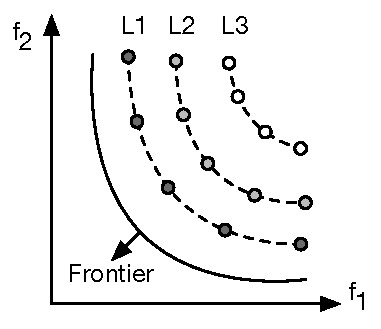
\includegraphics[width=0.2\textwidth]{figures/carbon_optimiser/paretofrontier/paretofrontier}
  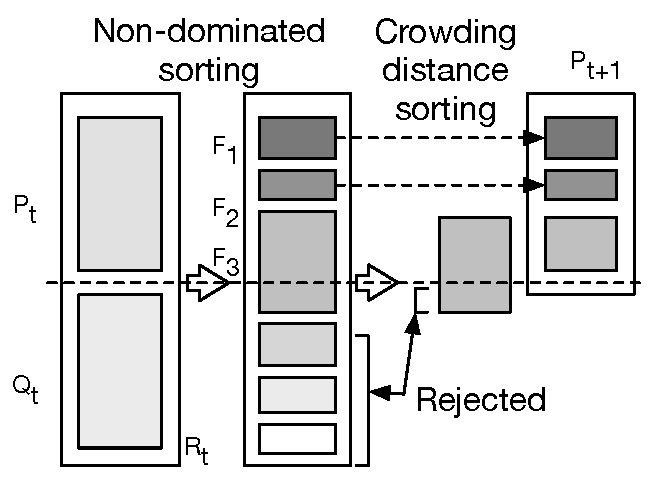
\includegraphics[width=0.270\textwidth]{figures/carbon_optimiser/algsketch/sketch2}
  \vskip -8pt
  \caption{a) Schematic of non-dominated sorting with solution layering b) Schematic of the NSGA-II procedure}
  \label{fig:pareto-layering}
  \vskip -15pt
\end{figure}


Next, each of the solutions are ranked according to their level of non-domination. An example of this ranking is shown in Figure \ref{fig:pareto-layering}a. Here, $f_1$ and $f_2$ are the objectives to be minimised. The Pareto front is the first front. All of the solutions in the Pareto front are not dominated by any other solution. The solutions in layer 1, L1, are dominated only by those in the Pareto front, and are non-dominated by those in L2 and L3.

The solutions are then ranked according to their layer. For example, the solutions in the Pareto front are given a fitness rank ($i_{rank}$) of 1, solutions in L1 have an $i_{rank}$ of 2, etc.

\subsubsection{Density Estimation}
($i_{distance}$) is calculated for each solution. This is the average distance between the two closest points to the solution in question. 


\subsubsection{Crowded comparison operator}
($\prec_n$) is used to ensure that the final frontier is an evenly spread out Pareto-optimal front. This is achieved by using the two attributes: $(i_{rank})$ and$(i_{distance})$. 
%\begin{enumerate}
%  \item Non-domination rank $(i_{rank})$
%  \item Local crowding distance $(i_{distance})$
%\end{enumerate}
The partial order is then defined as:\\	
$i\prec_nj$ if $(i_{rank}<j_{rank})$ or $((i_{rank}=j_{rank})$ and  $(i_{distance}>j_{distance}))$ \cite{Valkanas2014}.

This order prefers solutions with a lower rank $i_{rank}$. For solutions with the same rank, the solution in the less dense area is preferred.

\subsubsection{Main loop}

Similarly to the standard GA, a population $P_{0}$ is created with random parameters. The solutions of $P_0$ are then sorted according to non-domination. The child population $C'_{1}$ of size $N$ is then created by binary tournament selection, recombination and mutation operators. In this case, tournament selection is the process of evaluating and comparing the fitnesses of various individuals within a population. In binary tournament selection, two individuals are chosen at random, the fitnesses are evaluated and the individual with the better solution is selected~\cite{AbdRahman2016}. 



\begin{algorithm}[b]
\begin{algorithmic}[1]
\State $R_t=P_t \cup C'_t$ combine parent and child population
\State $\mathcal{F} = $ fast-non-dominated-sort $(R_t)$ 

where $\mathcal{F}=(\mathcal{F}_1, \mathcal{F}_2,\ldots)$
\State $P_{t+1}=\emptyset$
\While $\left|P_{t+1}<N\right|$
\State Calculate the crowding distance of $(\mathcal{F}_i)$)
\State $P_{t+1}=P_{t+1}\cup \mathcal{F}_i$
\EndWhile
\State Sort($P_{t+1}, \prec_n$) sort in descending order using $\prec_n$
\State $P_{t+1} = P_{t+1}[0:N]$ select the first $N$ elements of $P_{t+1}$
\State $Q_{t+1} = $ make-new-population$(P_{t+1})$ using 

selection, crossover and mutation to create 

the new population $Q_{t+1}$
\State $t=t+1$
\caption{NSGA-II main loop \cite{Valkanas2014}}
\label{algo:nsga2}
\end{algorithmic}
\end{algorithm}


Next, a new combined population is formed $R_{t}=P_{t} \cup C'_{t}$. $R_t$ has a size of $2N$. $R_t$ is then sorted according to non-domination. A new population is then formed $P_{t+1}$. Solutions are added from the sorted $R_t$ in order of non-domination. Solutions are added until the size of $P_{t+1}$ exceeds $N$. The solutions from the last layer are prioritised based on having the largest crowding distance~\cite{Valkanas2014}.

This process is shown in Figure \ref{fig:pareto-layering}b, which is repeated until the termination condition is met. A termination condition could be:  no significant improvement over $X$ iterations or a specified number of iterations have been performed. 



\section{Experimental Setup}
\label{sec:sim_environment}


\subsection{Simulation Environmental}
In order to evaluate the different carbon strategies we used the model developed by Kell \textit{et al}., ElecSim \cite{Kell,Kell2020}. ElecSim is an agent-based model which mimics the behaviour of decentralised electricity markets. For this paper, we have parametrised the model to data for the UK in 2018. This includes the power plants in operation in 2018, and the funds available to their respective companies \cite{dukes_511, companies_house}.

Five fundamental sections make up ElecSim: 1) power plant data; 2) scenario data; 3) the time-steps of the algorithm; 4) the power exchange; 5) the investment algorithm and 6) the generation companies (GenCos) as agents. ElecSim uses a subset of representative days of electricity demand, solar irradiance and wind speed to approximate a full year. In this context, representative days are a subset of days which when scaled up can adequately represent a year. 

Figure \ref{fig:model_details} details how these parts interact.

\begin{figure}
\centering
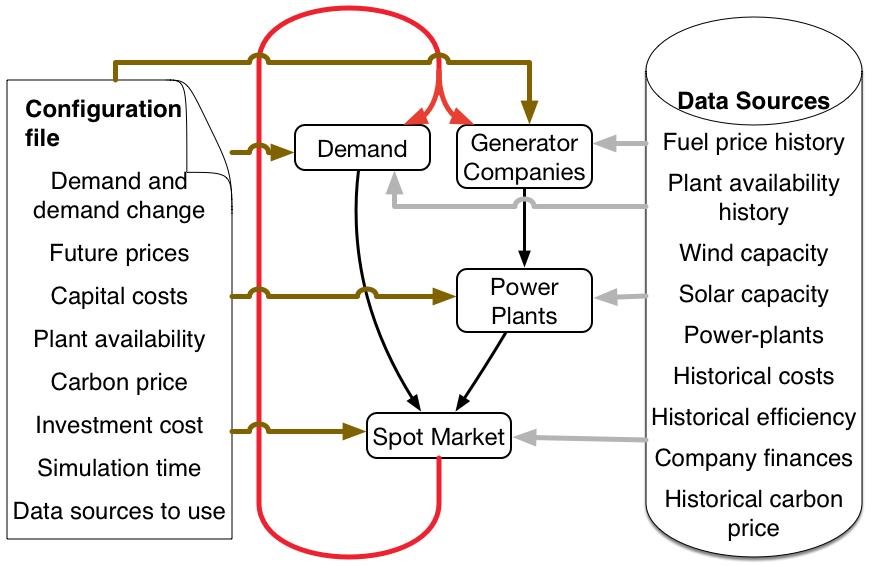
\includegraphics[width=0.49\textwidth]{/Users/b1017579/Documents/PhD/Projects/10-ELECSIM/run/carbon_tax_optimiser/figures/simulation_details/System_overview_large.png}
\caption{System overview of ElecSim.}
\label{fig:model_details}
\end{figure}

The market runs in merit-order dispatch and bids are made by the power plant's short-run marginal cost (SRMC). Investment in power plants are based upon a net present value (NPV) calculation. NPV is able to evaluate and compare investments with cash flows spread over many years. This is shown formally in Equation \ref{eq:npv_eq}, where $t$ is the year of the cash flow, $i$ is the discount rate, $N$ is the total number of years, or lifetime of power plant, and $R_t$ is the net cash flow of the year $t$:

\begin{equation} \label{eq:npv_eq}
NPV(i, N) = \sum_{t=0}^{N}\frac{R_t}{(1+t)^t}.
\end{equation}

The yearly income for each power plant is estimated for each generation company by running a merit-order dispatch electricity market 10 years into the future. However, the expected cost of electricity 10 years into the future is uncertain. We therefore use the reference scenario projected by BEIS and use the predicted costs of electricity calibrated by Kell \textit{et al} \cite{DBEIS2019, Kell2020}.



\subsection{Optimization}
\label{ssec:optimization}
\subsubsection{Non-parametric carbon policy}
\label{sssec:non_parametric_strategy}
The optimization approach took two stages. Firstly, we initialized the population of the NSGA-II algorithm $P_0$ with 18 attributes. These corresponded to a separate carbon tax for each year, shown by Equation \ref{eq:eighteen_degrees_freedom}:

\begin{equation}
\label{eq:eighteen_degrees_freedom}
	P_0=\{a_1,a_2,\ldots,a_{18}\}\\
\end{equation} 
\begin{equation*}
		 0\leq a_y\leq 250
\end{equation*}

\noindent where $P_0$ is the first population, $a_y$ is the attribute or carbon price in year $y$ and $a_1$ is the carbon price in year 1, $a_2$ the carbon price in year 2 and so forth. Each of the carbon prices were bound between the values of \textsterling$0$ and  \textsterling$250$ . This provided the optimization algorithm with the highest degree of freedom. This high degree of freedom enabled a high number of strategies to be trialled due its non-parametric nature. This, however, came with a large search space requiring a large number of iterations.


 \subsubsection{Linear carbon policy}
 \label{sssec:linear_carbon_strategy}
 To reduce the search space for the carbon strategy, we trialled a linear carbon strategy, of the form:
 \begin{equation}
 	p_c=a_1y_t+a_2
 \end{equation}
 \begin{equation*}
 	-14 \leq a_1\leq 14
 \end{equation*}
  \begin{equation*}
 	0 \leq a_2\leq 250
 \end{equation*}
 
 \noindent where $p_c$ is the carbon price, $y_t$ is the year, $m$ is the gradient or first attribute and $c$ is the intercept or second attribute. $a_1$ was bound by $-14$ and $14$, and $a_2$ by 0 and 250. These bounds were chosen to ensure that the carbon price did not exceed ${\sim}$\textsterling500 in the year 18 (2035) and was greater than ${\sim}$-\textsterling250, as well as ensuring that the carbon tax in the first year was greater than \textsterling0 but smaller than \textsterling250.

\section{results}
\label{sec:results}

In this section we explore the results of the optimisations, the optimum carbon strategies and the resultant electricity mixes.

\subsection{Non-parametric carbon policy}
\label{sssec:result_non_parametric_strategy}

Figure \ref{fig:free_points_ga_development} shows the development of the genetic algorithm against the rewards, relative carbon density and average electricity price. Darker colours display higher generation numbers. The first generation shows a wide spread in relative carbon density and average electricity price. However, over successive generations the solutions converge to a relative carbon density of 0 and an average electricity price under ${\sim}$\textsterling10MW/h. 

Strikingly, the rewards of relative carbon density and average electricity price are not mutually destructive. This could be due to the low short-run marginal cost of renewable energy which reduces both electricity prices and carbon emissions.



\begin{figure}
\centering
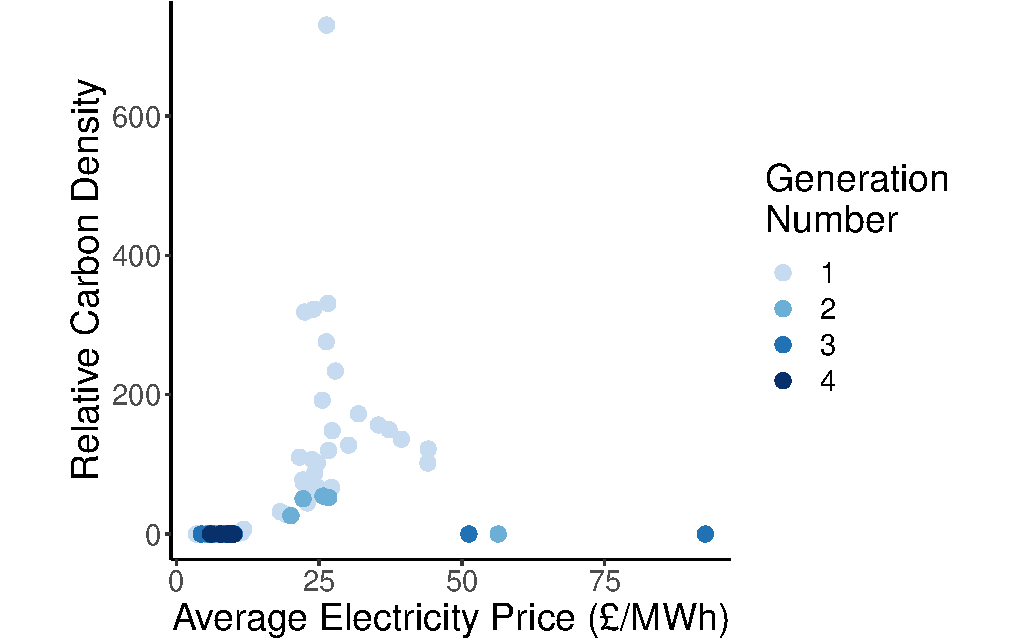
\includegraphics[width=0.4\textwidth]{/Users/b1017579/Documents/PhD/Papers/6-carbon-optimiser/acmart-master/samples/figures/results/free_points_ga_development}
\caption{Development of genetic algorithm rewards of average electricity price and relative carbon density in 2035 over time for non-parametric carbon policy.}
\label{fig:free_points_ga_development}
\end{figure}

To understand the optimum carbon strategies we visualised the parameters that produced the lowest average electricity prices in Figure \ref{fig:heatmap_of_free_points}. Specifically, we filtered for electricity prices under \textsterling5/MWh and displayed the results using a heat map. The darker colours represent a higher density of points. 

Figure \ref{fig:heatmap_of_free_points} displays a general trend, where carbon tax starts at ${\sim}$\textsterling100 until the year ${\sim}$2030, where it increases to ${\sim}$\textsterling200 by 2035. This may be due to the fact that a lower initial carbon tax of ${\sim}$\textsterling100 encourages investment in low-carbon technologies  before the higher rate of ${\sim}$\textsterling200 comes into force. This higher rate of carbon tax would allow GenCos to outcompete higher carbon emitting generators over the lifetime of the plants.

\begin{figure}
\centering
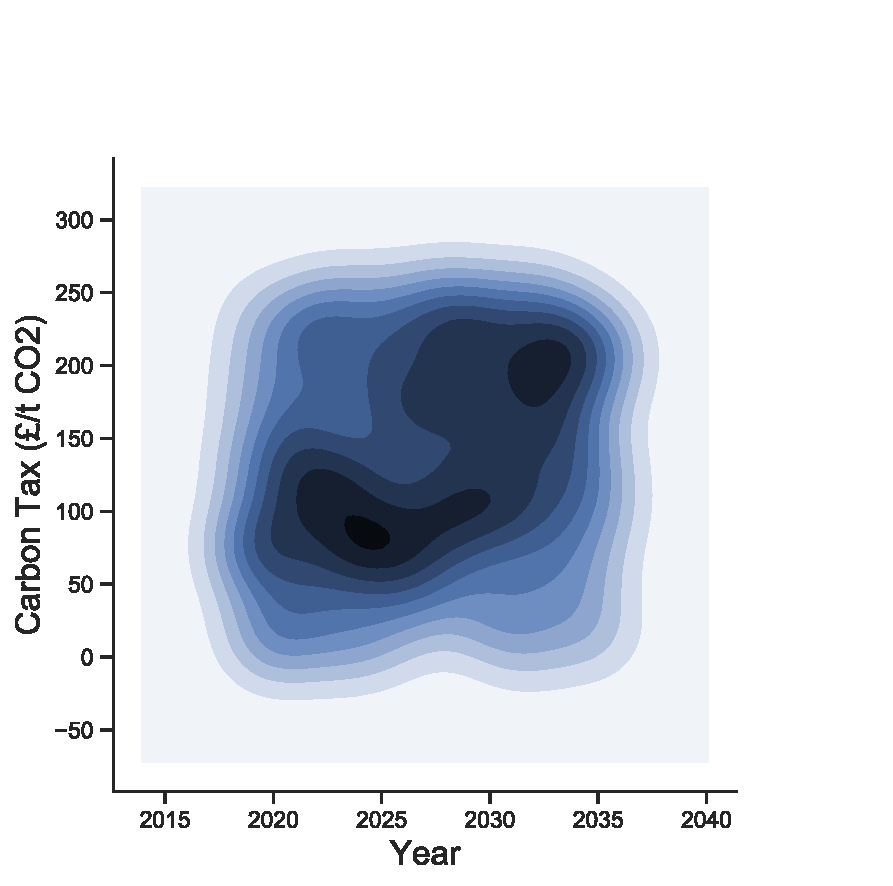
\includegraphics[width=0.35\textwidth]{/Users/b1017579/Documents/PhD/Papers/6-carbon-optimiser/acmart-master/samples/figures/results/best_heatmap_no_marginals}
\caption{2D density plot of non-parametric carbon tax policy that led to an average electricity price of below \textsterling5/MWh by 2035.}
\label{fig:heatmap_of_free_points}
\end{figure}

%\begin{figure}[width=0.49\textwidth]
%\centering
%\begin{subfigure}{.5\linewidth}
%  \centering
%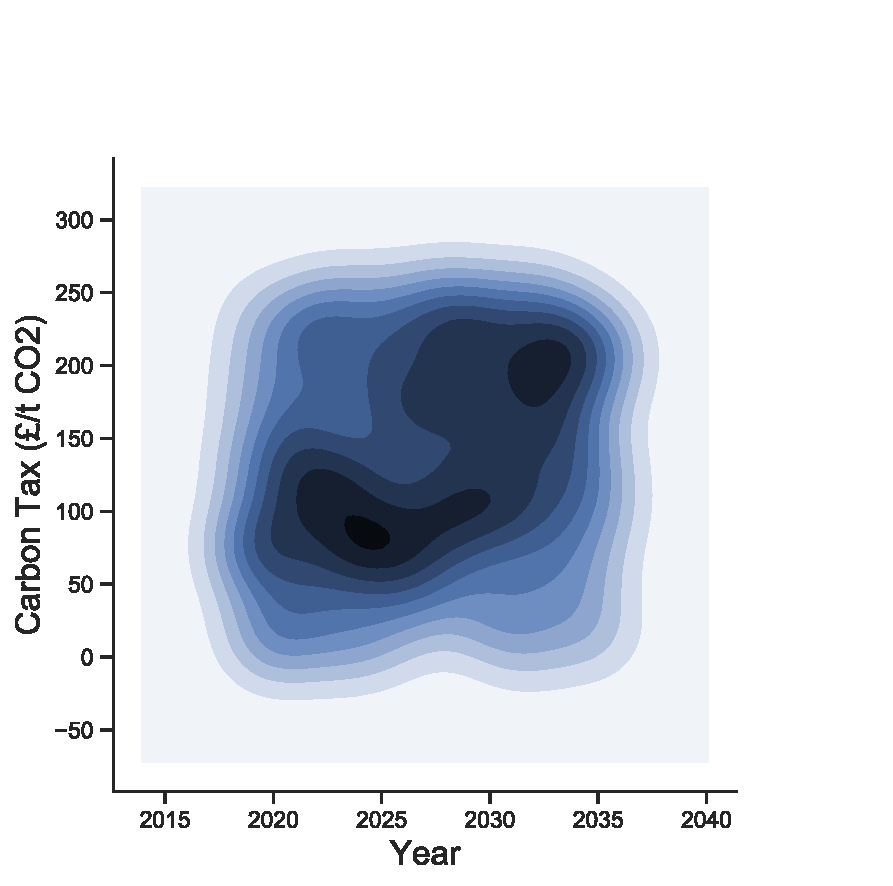
\includegraphics[width=.45\linewidth]{/Users/b1017579/Documents/PhD/Papers/6-carbon-optimiser/acmart-master/samples/figures/results/best_heatmap_no_marginals}
%%\caption{2D density plot of non-parametric carbon tax policy that led to an average electricity price of below \textsterling5/MWh by 2035.}
%\caption{2D density plot.}
%\label{fig:heatmap_of_free_points}\hspace*{-0.9em}
%\end{subfigure}%
%\begin{subfigure}{.5\linewidth}
%  \centering
%  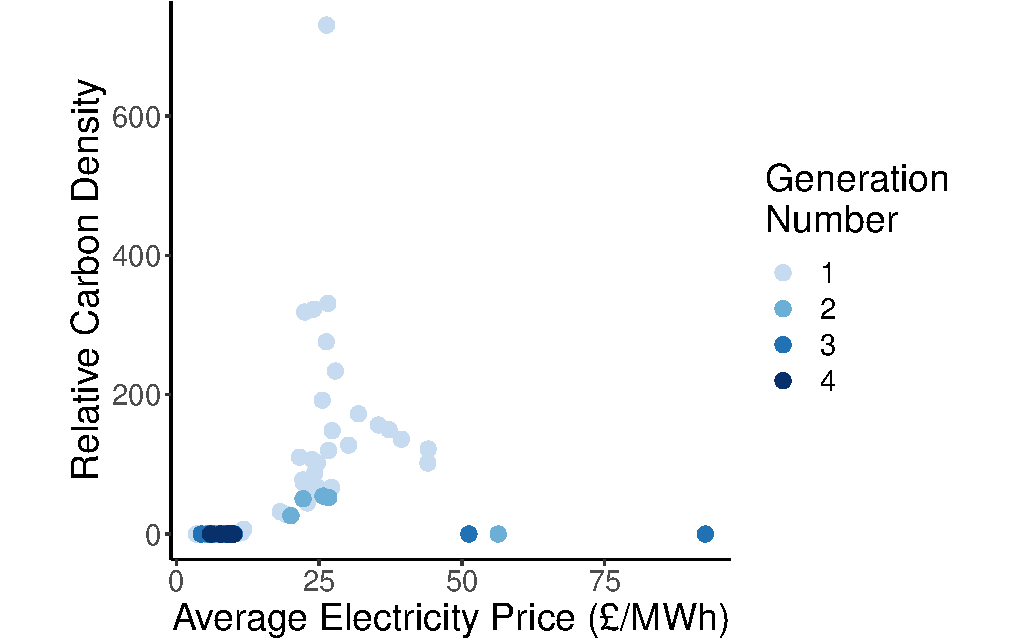
\includegraphics[width=.45\linewidth]{/Users/b1017579/Documents/PhD/Papers/6-carbon-optimiser/acmart-master/samples/figures/results/free_points_ga_development}
%%   \caption{Development of genetic algorithm rewards of average electricity price and relative carbon density in 2035 over time for highest degrees of freedom per year.}
%   \caption{Development.}
%   \label{fig:free_points_ga_development}
%\end{subfigure}
%\caption{A figure with two subfigures}
%\label{fig:test}
%\end{figure}






\subsection{Linear carbon policy}
\label{sssec:result_linear_carbon_strategy}

Figure \ref{fig:linear_ga_development} displays the development of the genetic algorothm against the rewards: relative carbon density and average electricity price. Similarly to the non-parametric carbon policy shown in Figure \ref{fig:free_points_ga_development}, the first generation shows a wide spread of results. However, the spread is smaller than that of the linear carbon policy. This may be due to the fact that it is easier for the GenCos to predict the carbon policy, which increases confidence in the NPV calculations. The linear carbon policy also converges to a relative carbon density of 0, and an average electricity price of ${\sim}<10$.

Figure \ref{fig:comparison_of_distributions} compares the distributions of average electricity price for both techniques. Both methods show improvements as the number of generations of the genetic algorithm increase.  The linear policy, however, is able to more quickly converge to a low average electricity price, with a mode of ${\sim}$\textsterling5.4MW/h. The non-parametric policy has a number of poorer performing parameters, and Generation Number 4 has a bimodal distribution, with a mode of ${\sim}$\textsterling6.3MW/h.

\begin{figure}
\centering
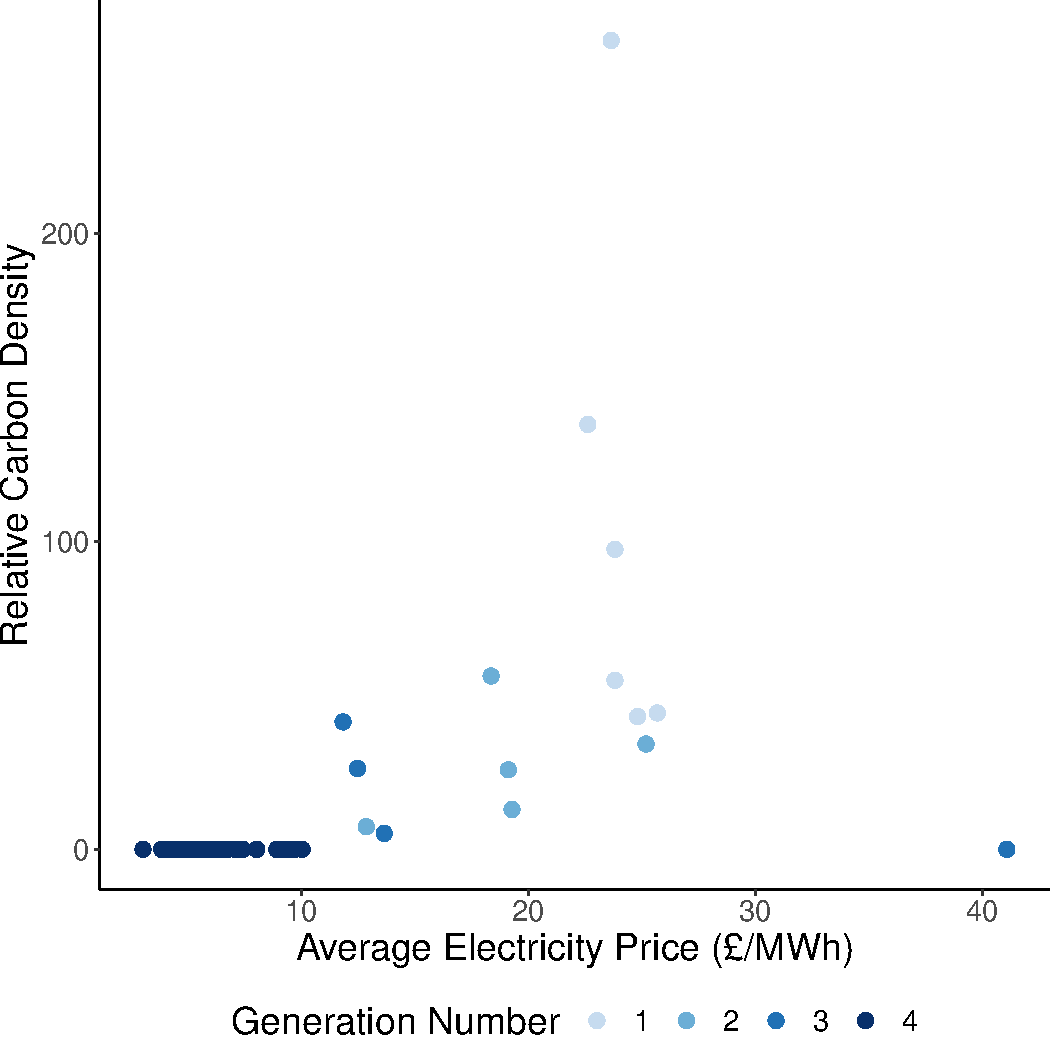
\includegraphics[width=0.4\textwidth]{/Users/b1017579/Documents/PhD/Papers/6-carbon-optimiser/acmart-master/samples/figures/results/linear_ga_development.pdf}
\caption{Development of genetic algorithm rewards of average electricity price and relative carbon density in 2035 over time for linear carbon strategy.}
\label{fig:linear_ga_development}
\end{figure}


%\begin{figure}
%\centering
%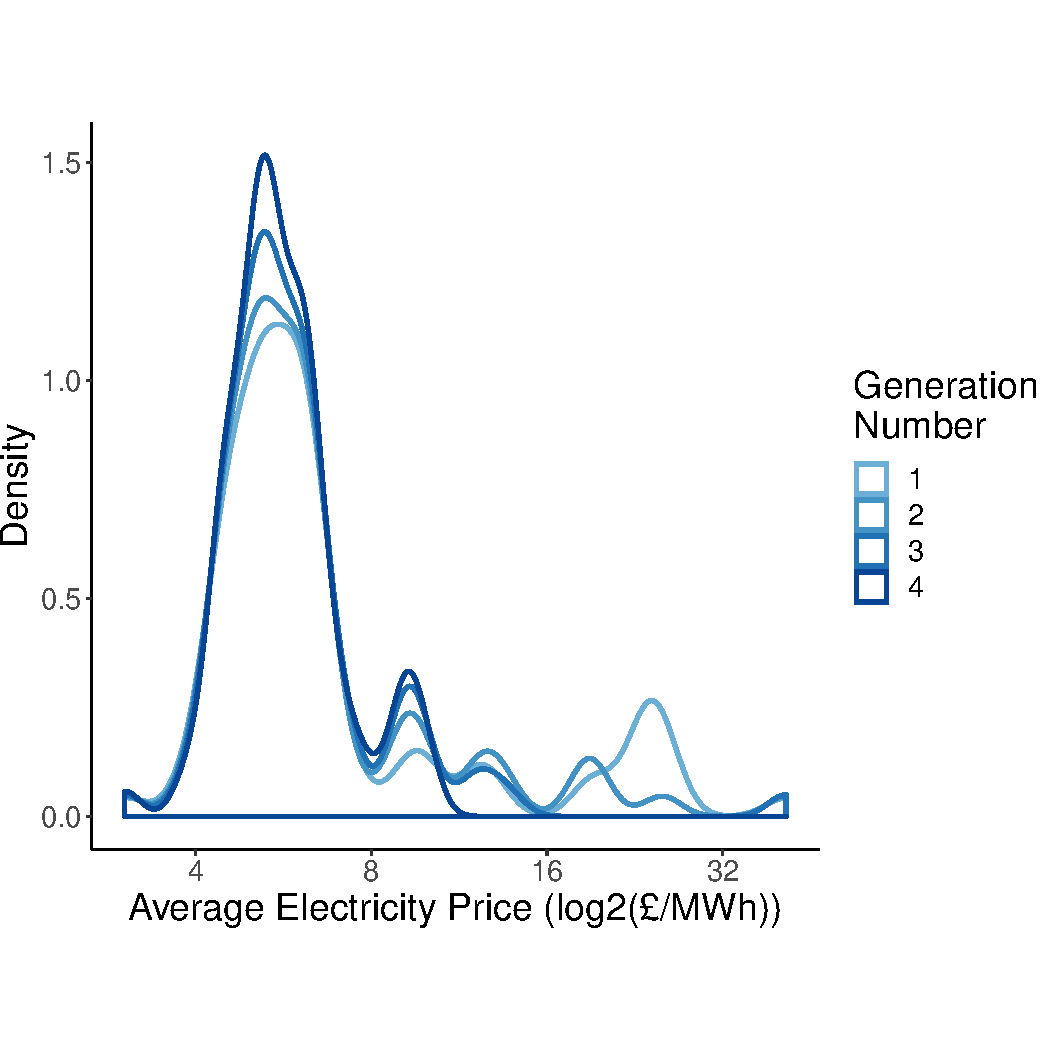
\includegraphics[width=0.49\textwidth,]{/Users/b1017579/Documents/PhD/Papers/6-carbon-optimiser/acmart-master/samples/figures/results/linear_ga_development_distribution_avg_elec_price}
%\caption{Density plot of average electricity price in 2035 over generation number of genetic algorithm.}
%\label{fig:forward_scenario_best_pdcs}
%\end{figure}



\begin{figure}
\centering
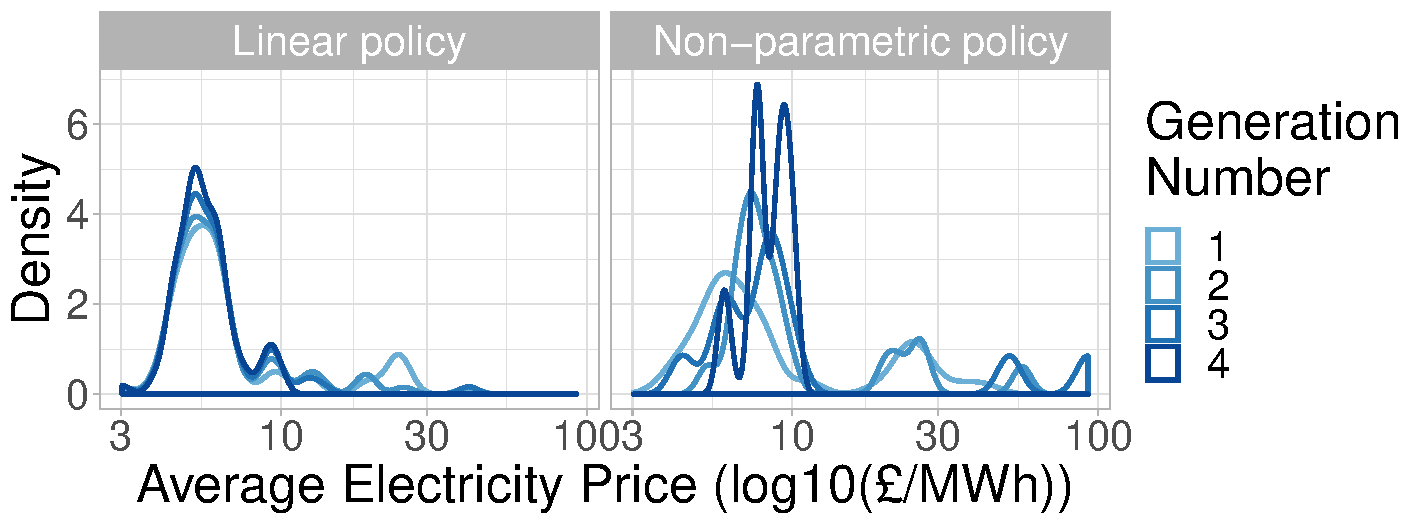
\includegraphics[width=0.49\textwidth,]{/Users/b1017579/Documents/PhD/Papers/6-carbon-optimiser/acmart-master/samples/figures/results/linear_and_free_ga_development_distribution_avg_elec_price.pdf}
\caption{Density plot of average electricity price in 2035 over generation number of genetic algorithm for both linear and non-parametric policy.}
\label{fig:comparison_of_distributions}
\end{figure}

Figure \ref{fig:linear_actual_pdcs} displays the linear carbon policies which had an average electricity price under \textsterling4.5MW/h. There is not a single `optimum' carbon policy, with a range of policies exhibited. 

\begin{figure}
\centering
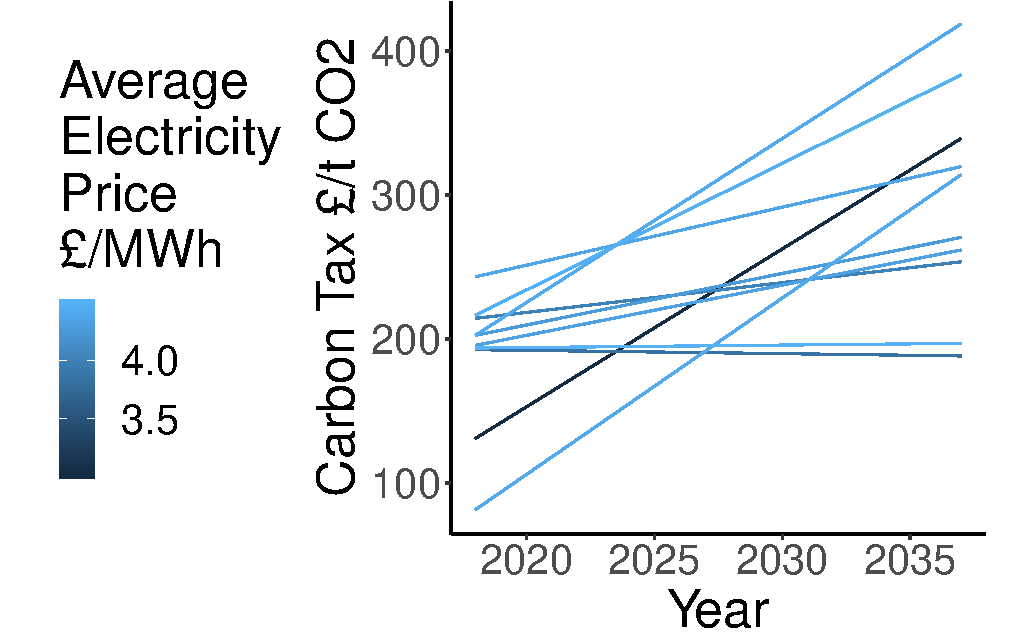
\includegraphics[width=0.4\textwidth]{/Users/b1017579/Documents/PhD/Papers/6-carbon-optimiser/acmart-master/samples/figures/results/linear_actual_lines}
\caption{Linear carbon policies under \textsterling4.5MW/h visualised.}
\label{fig:linear_actual_pdcs}
\end{figure}

\begin{figure}
\centering
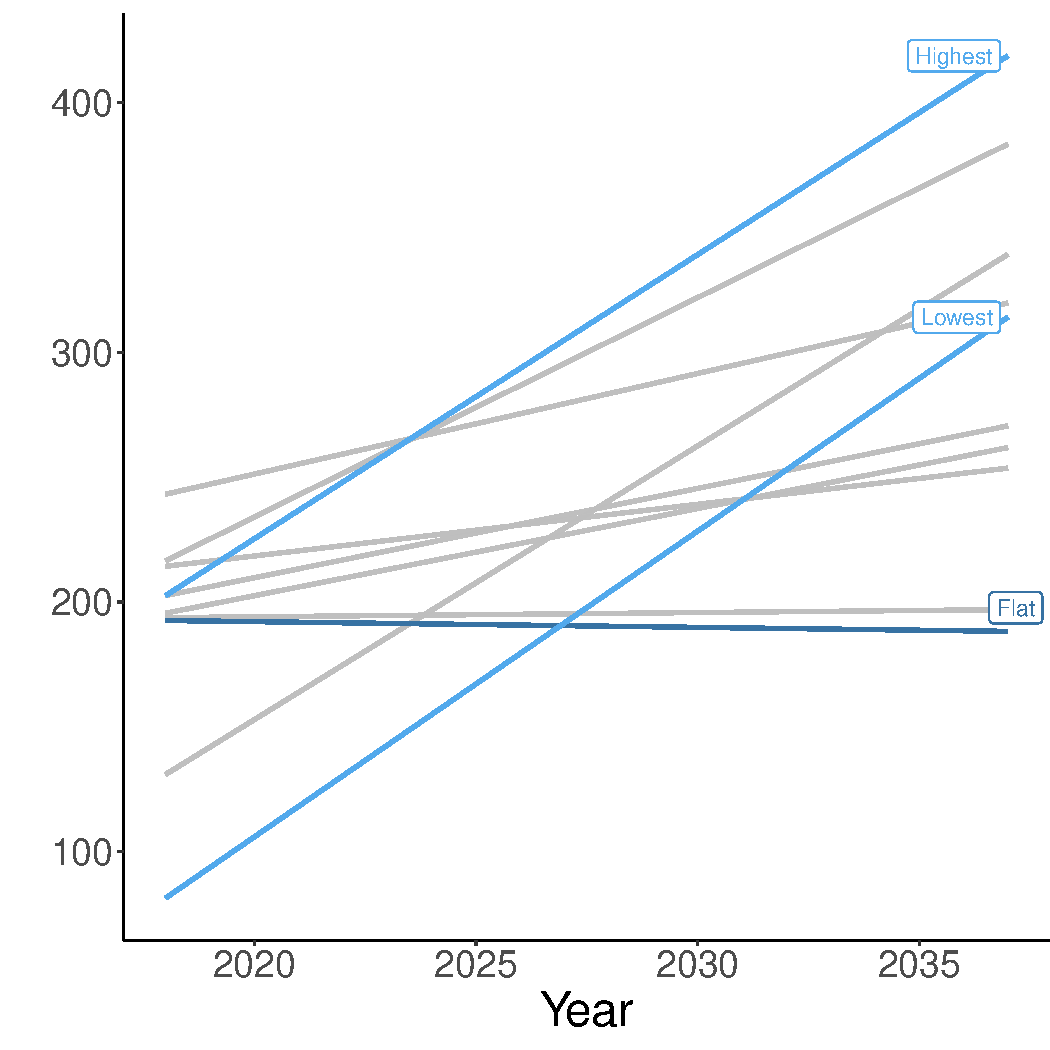
\includegraphics[width=0.3\textwidth]{/Users/b1017579/Documents/PhD/Papers/6-carbon-optimiser/acmart-master/samples/figures/results/highlighted_linear_actual_lines}
\caption{Highlighted inear carbon policies under \textsterling4.5MW/h.}
\label{fig:highlighted_linear_actual_pdcs}
\end{figure}


\begin{figure*}
\centering
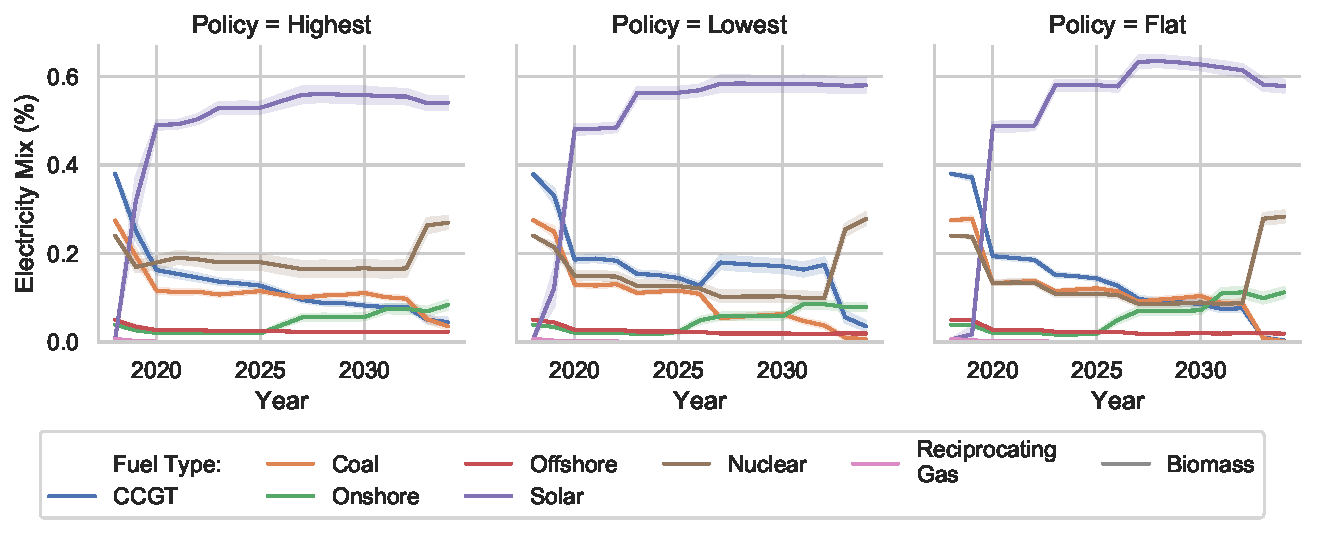
\includegraphics[width=0.95\textwidth]{/Users/b1017579/Documents/PhD/Papers/6-carbon-optimiser/acmart-master/samples/figures/results/best_electricity_mixes_facet}
\caption{Electricity mixes under selected linear carbon policies.}
\label{fig:best_electricity_mixes_facet}
\end{figure*}



%lowest_data_mix.pdf
%flat_data_mix
%highest_data_mix



\section{Conclusion}
\label{sec:conclusion}
Placeholder

%\section{Acknowledgments}



%\begin{acks}
%Anonymized
%%This work was supported by the Engineering and Physical Sciences Research Council, Centre for Doctoral Training in Cloud Computing for Big Data [grant number EP/L015358/1].
%\end{acks}

%%
%% The next two lines define the bibliography style to be used, and
%% the bibliography file.
\newpage
\bibliographystyle{ACM-Reference-Format}
\bibliography{library,custombibtex}

%%
%% If your work has an appendix, this is the place to put it.
\appendix


\end{document}
\endinput
%%
%% End of file `sample-sigconf.tex'.
